% Latex template: mahmoud.s.fahmy@students.kasralainy.edu.eg
% For more details: https://www.sharelatex.com/learn/Beamer

\documentclass[aspectratio=169]{beamer}            % Document class

\usepackage[portuguese]{babel}          % Set language
\usepackage[utf8x]{inputenc}            % Set encoding
\usepackage{courier}
\mode<presentation> {                   % Set options
  \usetheme{default}                    % Set theme
  \usecolortheme{default}               % Set colors
  \usefonttheme{default}                % Set font theme
  \setbeamertemplate{caption}[numbered]	% Set caption to be numbered
}

\setbeamertemplate{navigation symbols}{}
\setbeamertemplate{footline}[frame number]
\setbeamercovered{transparent}

\newcommand\Wider[2][3em]{%
\makebox[\linewidth][c]{%
  \begin{minipage}{\dimexpr\textwidth+#1\relax}
  \raggedright#2
  \end{minipage}%
  }%
}

% Uncomment this to have the outline at the beginning of each section highlighted.
%\AtBeginSection[]
%{
%  \begin{frame}{Outline}
%    \tableofcontents[currentsection]
%  \end{frame}
%}

\usepackage{graphicx}                   % For including figures
\usepackage{booktabs}                   % For table rules
\usepackage{hyperref}                   % For cross-referencing
\usepackage{caption}
\usepackage{siunitx}% Allows more control over captions in figs and tables


\title{Revisão de Atividades da FAC}	% Presentation title
%\author{Author One}					% Presentation author
\institute{LNLS.DAC.FAC}				% Author affiliation
\date{2024-07-12 -- 2024-08-23}			% Today's date


% Machine studies in the period
% =============================

% 2024-07-16-SI_60hz_ff_orbit
% 2024-07-18-SI_bpm02C1_1_oscillations
% 2024-07-22-AS_machine_characterization_screens_images
% 2024-07-22-SI_acquisition_ORION_concrete
% 2024-07-28-AS_machine-shutdown



\begin{document}

\begin{frame}
  \titlepage
  \href{https://github.com/lnls-fac/doc-review-dac-fac}{\beamergotobutton{Link para o repo github desta apresentação: https://github.com/lnls-fac/doc-review-dac-fac}}
  \href{https://www.overleaf.com/read/sbdjxtzfchrm}{\beamergotobutton{Link para o projeto overleaf destas notas}}
\end{frame}

\begin{frame}{Outline}
  \tableofcontents
\end{frame}

\section{Caracterização da Máquina - Pré-parada}

% 2024-07-22-AS_machine_characterization_screens_images


\begin{frame}{Caracterização da Máquina - Pré-parada}

{\footnotesize
% \vspace{-0.3cm}
\begin{itemize}
    % \setlength\itemsep{1em}
    \item estudo dia 2024-07-22
\end{itemize}
}
% % \vspace{-0.2cm}
% \begin{figure}[ht]
%     \begin{minipage}[b]{0.4\linewidth}
%         \centering
%         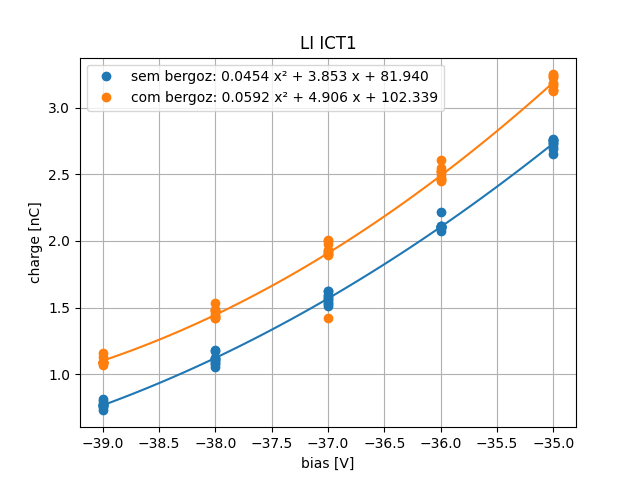
\includegraphics[width=\textwidth]{2024-07-12/figures/li-ict1.png}
%         \caption{Calibration of LI ICT1.}
%         \label{fig:a}
%     \end{minipage}
%     \hspace{0.2cm}
%     \begin{minipage}[b]{0.4\linewidth}
%         \centering
%         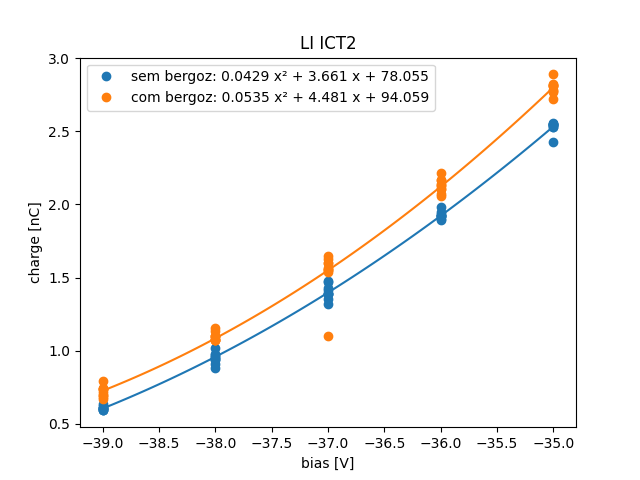
\includegraphics[width=\textwidth]{2024-07-12/figures/li-ict2.png}
%         \caption{Calibration of LI ICT2.}
%         \label{fig:b}
%     \end{minipage}
% \end{figure}
\end{frame}

\section{FF de órbita para perturbação em 60 Hz}

% 2024-07-16-SI_60hz_ff_orbit

\begin{frame}{FF de órbita para perturbação em 60 Hz}

{\footnotesize
\begin{itemize}
    \setlength\itemsep{0.5em}
    \item estudos em 2024-05-14 e 2024-07-01 \href{https://ais-eng-srv-ta.cnpem.br/Olog/index.html\#22801\_4}{\beamergotobutton{Olog \#22801\_4}}
    \item no primeiro estudo, apenas caracterização do FF, sem SOFB.
    \item no segundo estudo testamos nova versão do SOFB com as corretoras no modo \ot{RmpWfm} e agindo no \it{WfmOffsetKick}.
\end{itemize}
}
\vspace{-0.2cm}
\centering
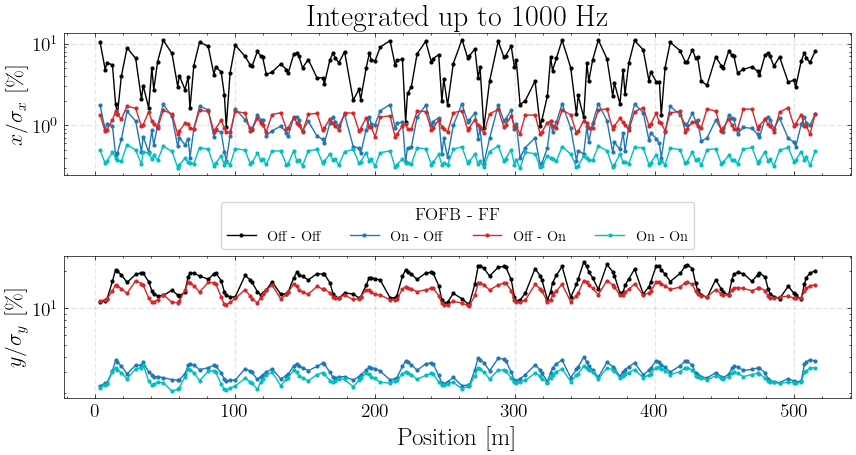
\includegraphics[width=0.7\linewidth]{2024-07-12/figures/integrated_distortion_up_to_1000Hz_run2.png}
\end{frame}

% \section{Estimativa de corrente máxima}

% * 2024-05-13-SI_max_stored_current_estimate (maximum-beam-current-estimate)


\begin{frame}{Estimativa de corrente máxima}

{\footnotesize
\begin{itemize}
    % \setlength\itemsep{1em}
    \item estudo dia 2024-05-13 \href{https://cnpemcamp.sharepoint.com/:b:/s/FAC/EYc5lGyqOatKoH_Rp2DNA1oBWygwBlE_1N8TA8AZYdNcBw?e=wTYFhx}{\beamergotobutton{Teams FAC/Machine Studies/Files}}
    \item dois trens de pacotes centrados nos buckets 260 e 292, acumulando e acompanhando as temperaturas dos componentes do anel
    \item conseguimos chegar em 90 mA (equivalente a feixe uniforme de 220 mA) 
    \item sensor MD4 (bellows entre scraper vertical e dipolo) chegou a 49$^\circ$C
    \item top-up por 1h em 90 mA $\rightarrow$ 80 mA, mais tempo e MD4 foi para 47$^\circ$C
    \item 4 bellows do TR01 são elípticos, enquanto outros são circulares (estes não aqueceram).
    \item somente o MD4 aqueceu, outros 3 não: o MD4 deve ter alguma particularidade mecânica.
\end{itemize}
}
% \vspace{-0.3cm}
\begin{figure}[ht]
    \centering
    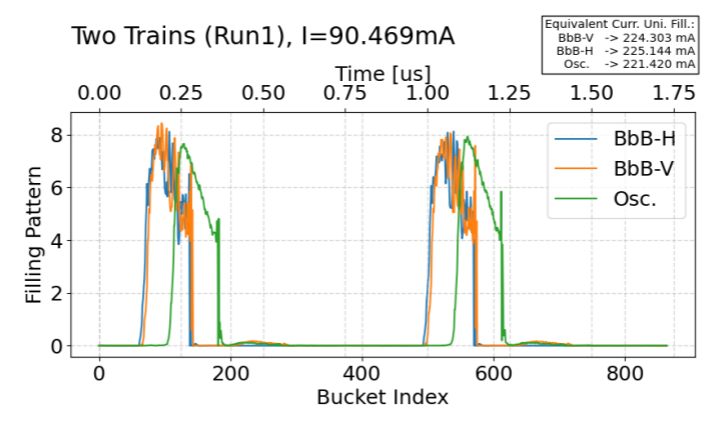
\includegraphics[height=3.2cm]{2024-07-12/figures/filling-pattern.png}
\end{figure}
\end{frame}
% \section{Ótica de dados TbT}

% 2024-05-21-SI_kickedbeam_tbt_acquisitions (tbt-acquisitions)
% 2024-06-11-SI_kickedbeam_tbt_acquisitions (tbt-acquisitions)


\begin{frame}{Ótica de dados TbT: Testes com pingers}

{\footnotesize
\begin{itemize}
    \item estudo dia 2024-05-21 \href{https://ais-eng-srv-ta.cnpem.br/Olog/index.html\#22749\_1}{\beamergotobutton{Olog \#22749\_1}}
    \item scan de delays dos pingers e testes de aquisição TbT
    \item amplitudes menores do que esperadas no feixe quando kickado pelos pingers
    \item desconfiando da temporização, fizemos scan dos \texttt{delay\_raw} para pingh e pingv
    \item delays ótimos encontrados, problema de amplitudes permaneceu
    \item realizamos aquisições varrendo kicks para levantar uma tabela de calibração 
    \item fator de calibração p/ (pingh, pingv) = (1.5417, 1.0227)
\end{itemize} 
}
\begin{figure}
    \centering
    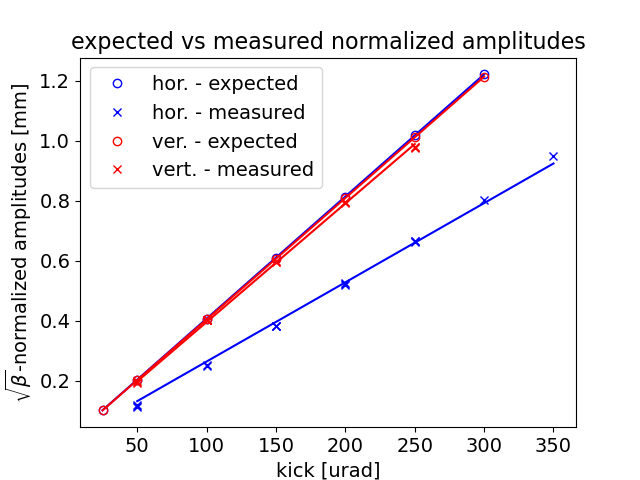
\includegraphics[scale=0.35]{2024-06-21/figures/norm_amp_expected_vs_observed-210524.png}
\end{figure}
\end{frame}



\begin{frame}{Ótica de dados TbT: Medidas de tune-shifts com amplitude}
\begin{minipage}{0.38\textwidth}
    {\footnotesize
    \begin{itemize}
        \item estudo dia 2024-06-11 \href{https://ais-eng-srv-ta.cnpem.br/Olog/index.html\#22749\_1}{\beamergotobutton{Olog \#22749\_1}}
        \item com pingers calibrados, realizamos aquisições TbT do feixe kickado
        \item tunes via espectro dos modos $U$ do SVD da matriz história de $N$ voltas nos 160 BPMs $$X = U \Sigma V^\intercal,  X = [[x_{ij}], [y_{ij}]] \in \mathbb{R}^{N\times 320}$$
    \end{itemize}
}    
\end{minipage}
\hfill
\begin{minipage}{0.58\textwidth}
    \centering
    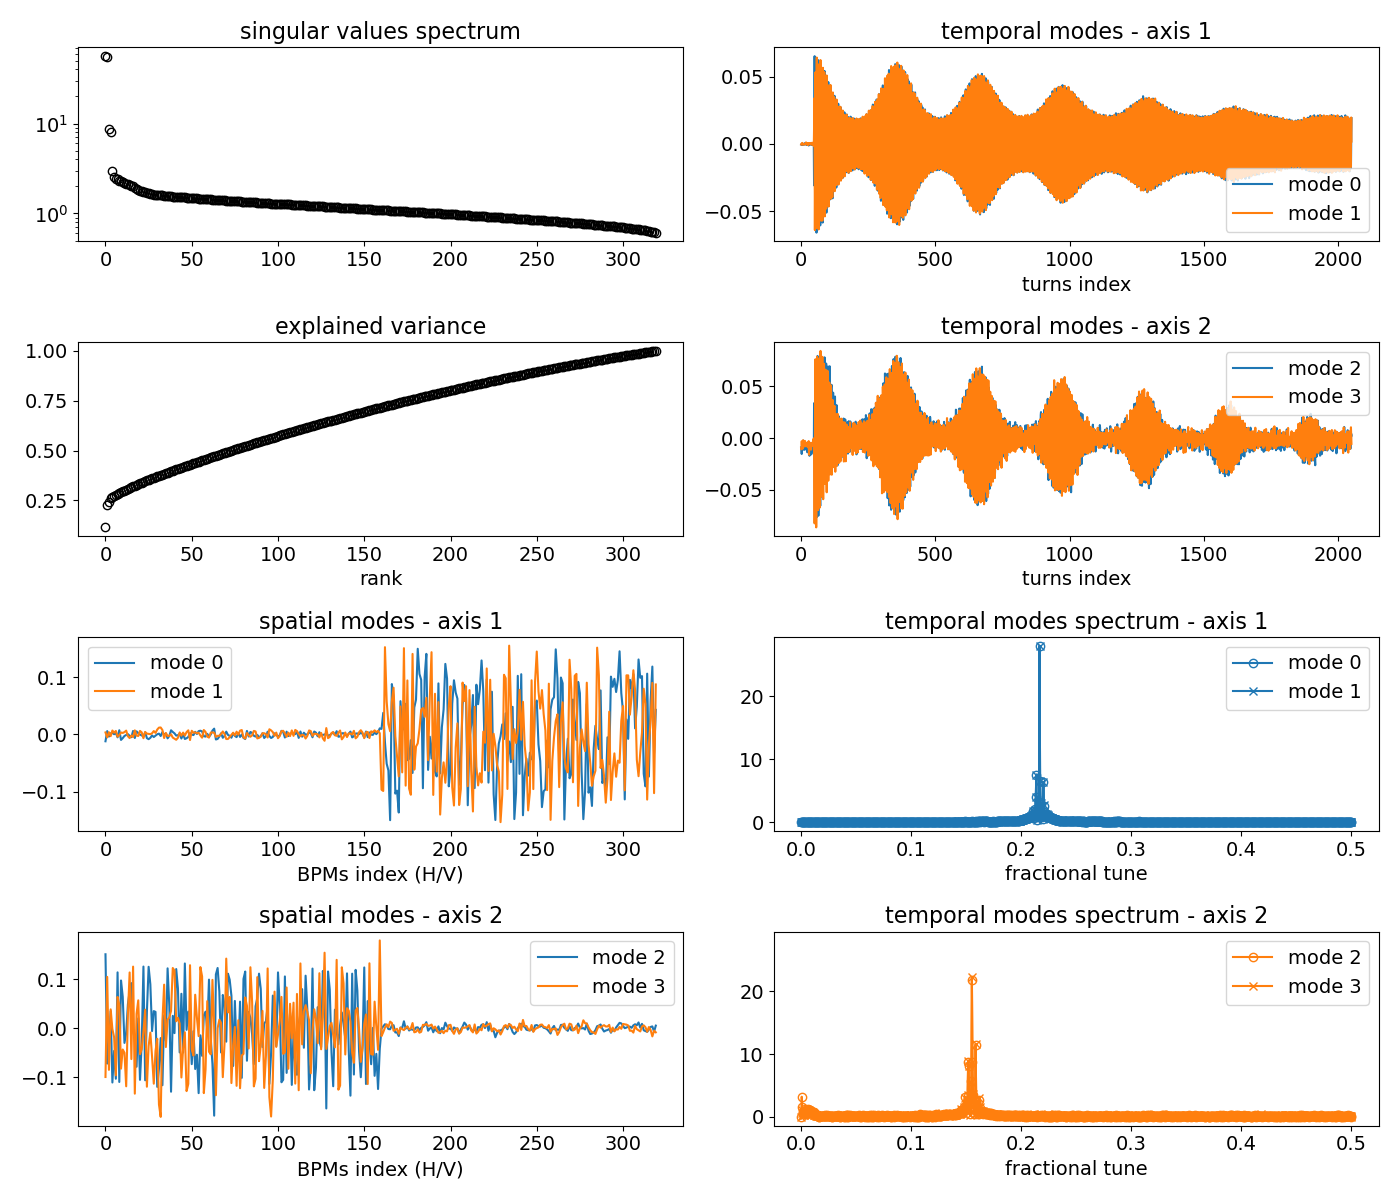
\includegraphics[width=\textwidth]{2024-06-21/figures/tbt_modal_analysis.png}
\end{minipage}
\end{frame}


\begin{frame}{Ótica de dados TbT: Tune-shifts, medidas vs. modelo}

{\footnotesize
\begin{itemize}
    \item regime de tune-shift com amplitude linear (kicks pequenos)
    \item como já esperado, nosso modelo da dinâmica não linear dnão descreve bem a máquina, após a otimização RCDS para novas sintonias.
\end{itemize}
}
\begin{figure}
    \centering
    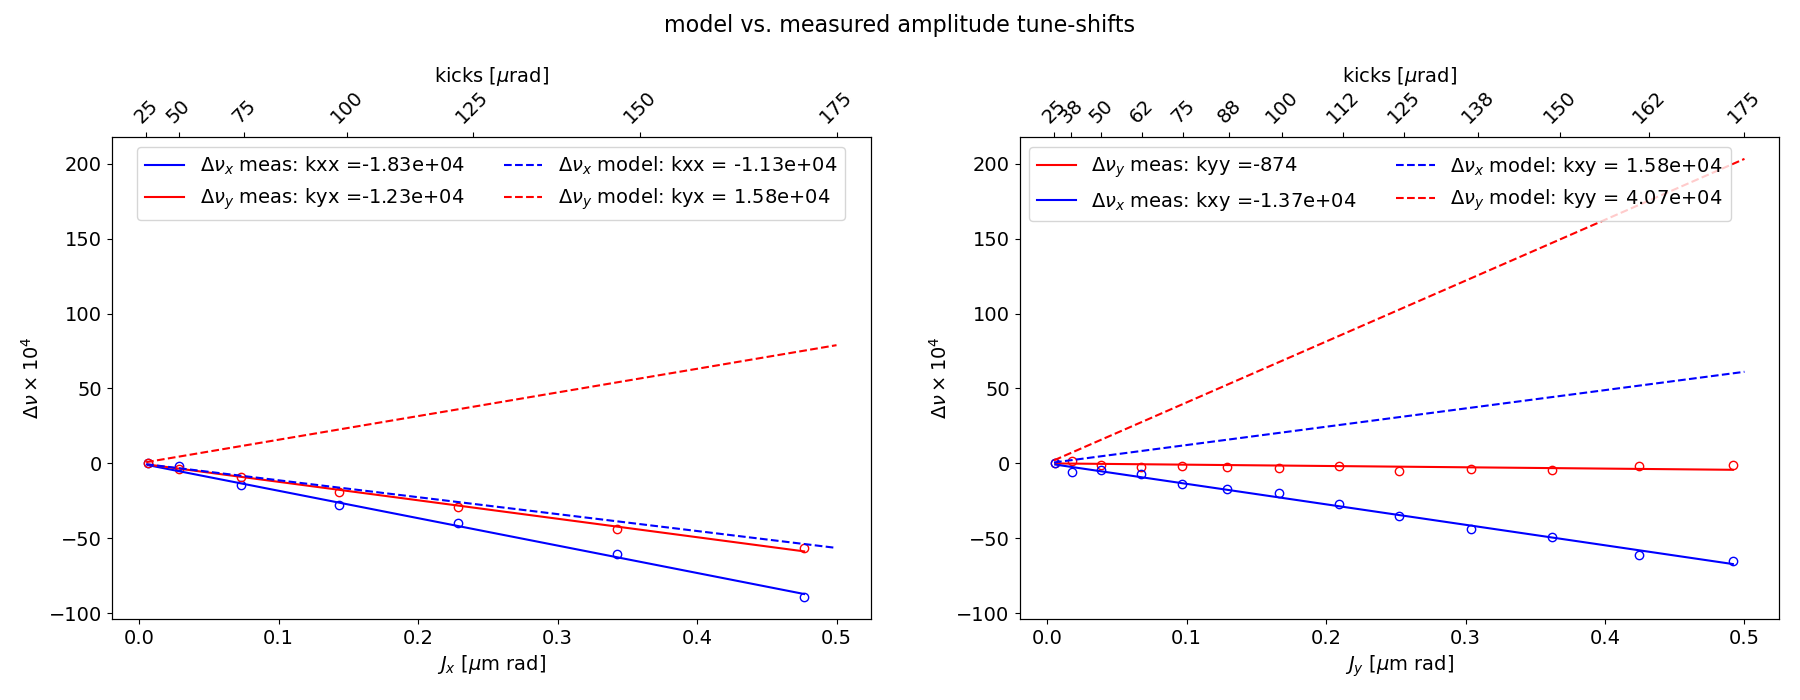
\includegraphics[scale=0.3]{2024-07-12/figures/model_vs_meas_adts.png}
\end{figure}

\end{frame}
% \section{Otimização do NLK}

% * 2024-05-14-SI_NLK (nlk)
% * 2024-05-21-SI_NLK (nlk)


\begin{frame}{Otimização do NLK}

\begin{itemize}
    \item Estudos em 2024-05-14 e 2024-05-21
    \item Dia 14: bumps para avaliar necessidade de realinhamento. $\Delta x = \SI{30}{\micro\meter}$
    \item Dia 20: parada, realinhamento de $\Delta x = \SI{22}{\micro\meter}$
    \item Dia 21: medida mostrou que menor distorção ocorre sem bump 
\end{itemize}
\vspace{1cm}
    \centering
    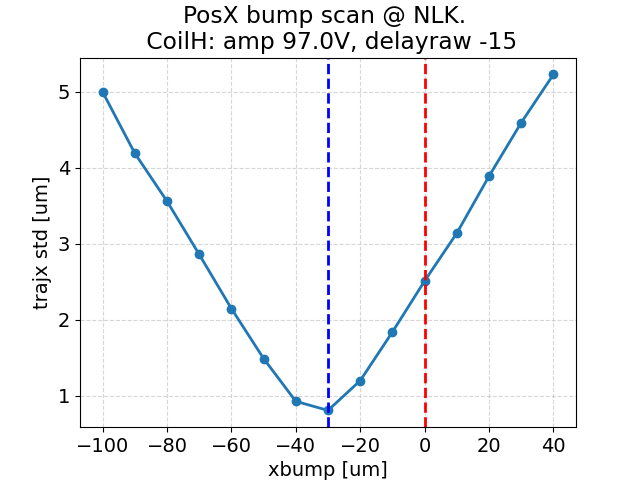
\includegraphics[width=0.27\textwidth]{2024-07-12/figures/NLK_scanbumpx_before_align.png}\hfill
    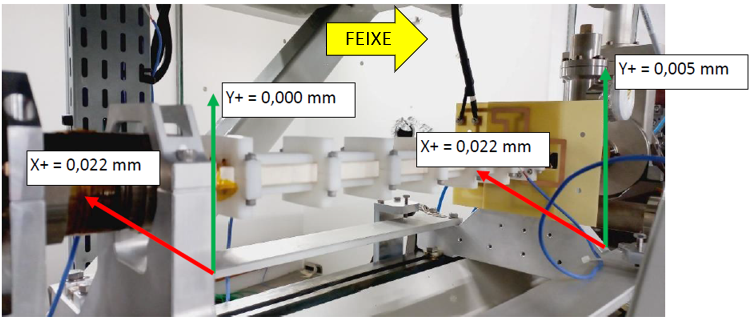
\includegraphics[width=0.45\textwidth]{2024-07-12/figures/NLK_align_May2024.png}\hfill
    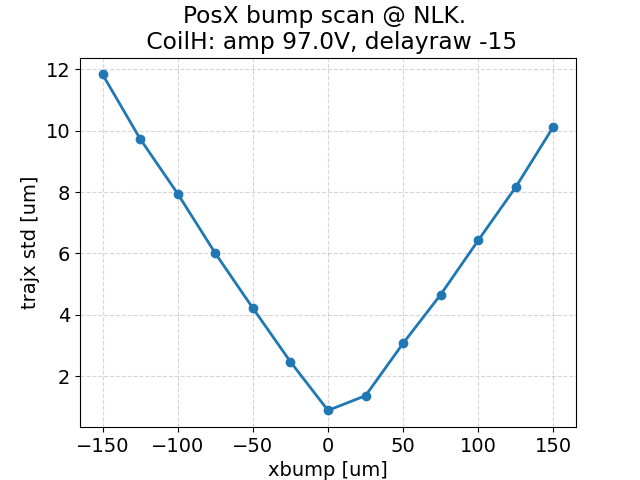
\includegraphics[width=0.27\textwidth]{2024-07-12/figures/NLK_scanbumpx_after_align.png}
\end{frame}

%  \section{Correção de órbita na rampa do booster}

% 2024-05-21-BO_ramp_orbcorr (boramp-orbit-correction)


\begin{frame}{Correção de órbita na Rampa do booster}
\begin{itemize}
    \setlength\itemsep{1em}
    \item Estudos 2024-05-21
\end{itemize}
\end{frame}

% \section{Otimização da injeção no Booster}

% * 2024-05-27-BO_injection_optimization (boinj-optimization)


\begin{frame}{Otimização da injeção no Booster}
\begin{itemize}
    \item estudo dia 2024-05-27 \href{https://ais-eng-srv-ta.cnpem.br/Olog/index.html\#22587\_6}{\beamergotobutton{Olog \#22587\_6}}
    \item pós-otimização de amplitude e fase do subharmonic buncher 
    \begin{itemize}
        \item a fase otimizada no SHB é tal que o beam loading afeta apenas a própria fase do sinal, e não a sua amplitude.
        \item com essas alterações, o feixe que chega ao BO mudou, e também a eficiência da rampa
    \end{itemize}
    \item otimização da corrente na rampa do BO à baixa energia usando o RCDS
    \item botões de otimização
    \begin{itemize}
        \item PosAng na TB, BOInjKicker, kly2 amp, kly2 phase (rodadas 1 e 2)
        \item PosAng na TB, BOInjKicker, kly2 amp, kly2 phase, RF bottom phase (rodada 3)
    \end{itemize}
    \item função objetivo: corrente à baixa energia (indice 60 da wfm da DCCT) 
\end{itemize}    
\end{frame}


\begin{frame}{Otimização da injeção no Booster}
\begin{itemize}
\item Resultados: 
\begin{itemize}
    \item Rodada 1: condições pré-otimização do SHB restauradas 
    \item Rodadas 2 e 3: Pouco progresso em relação à rodada 1.
\end{itemize}
\begin{figure}
    \centering
    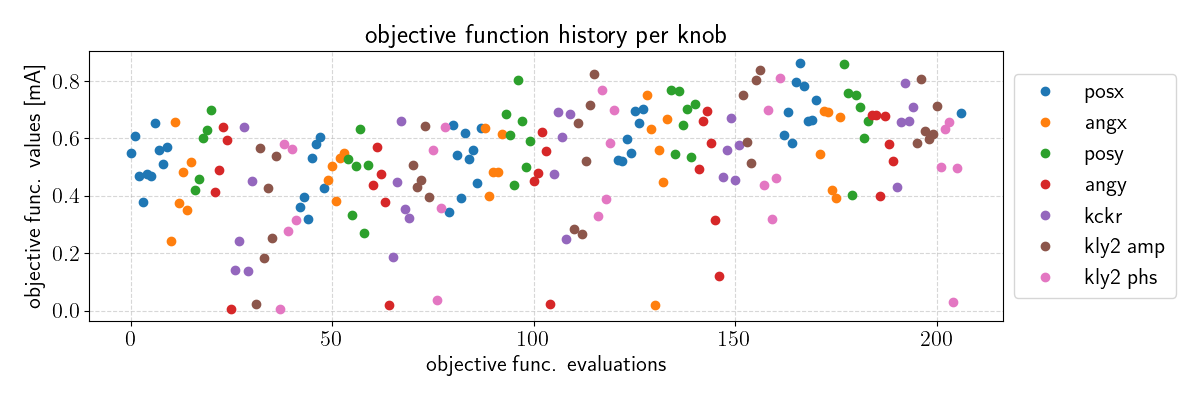
\includegraphics[width=\linewidth]{2024-07-12/figures/run1_history_by_knob.png}
    % \caption{Caption}
\end{figure}
\end{itemize}
\end{frame}

% \section{BBA}

% 2024-06-10-SI_bba
% 2024-06-16-SI_bba_tests
% 2024-06-17-SI_bba


\begin{frame}{BBA}
\vspace{-0.2cm}
{\footnotesize
\begin{itemize}
    \setlength\itemsep{0.5em}
    \item estudos em 2024-06-10, 2024-06-16 e 2024-06-17
    \item BBA do dia 05-10 com resultados estranhos: assinaturas da variação de órbita com delta negativo dos trims dos quads correspondiam distorções distribuídas.
    \item BBAs antes e depois da parada do dia 17: OK. Maior variação no 03M2 (cabo movimentado na parada para acomodar outros cabos da SRFCav)
    \item os problemas do dia 10 não voltaram a acontecer. não entendemos...
\end{itemize}
}
\centering
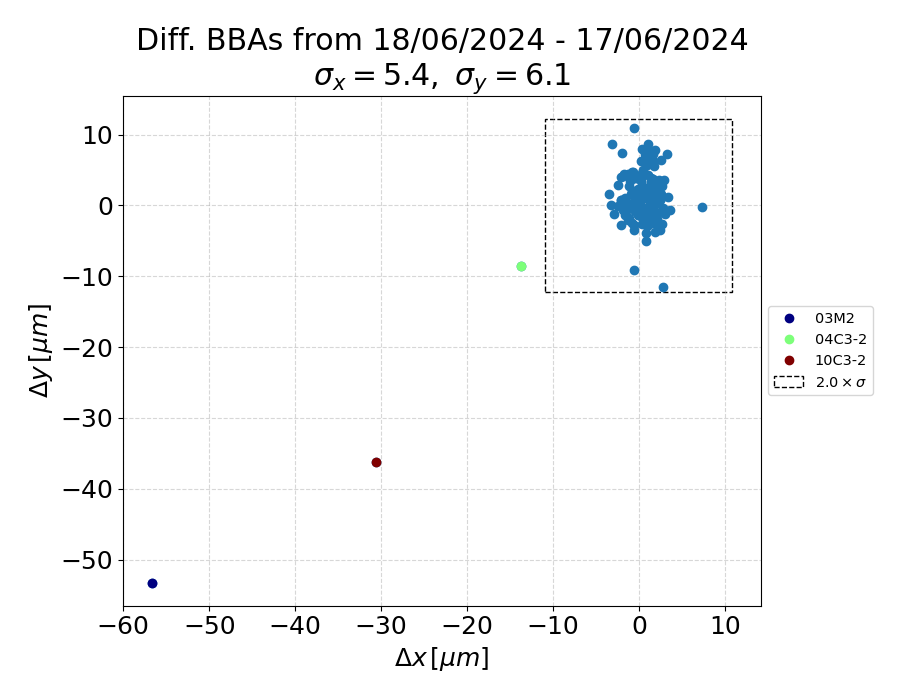
\includegraphics[width=0.4\linewidth]{2024-07-12/figures/diff_to_bba_orb_before_2024_06_17_shutdown.png}
\end{frame}
% \section{Bump de órbita no booster}

% * 2024-06-18-BO_optimization (boorb_bumps)


\begin{frame}{Bump de órbita no booster: bumps X adicionais de órbita no trecho}
\begin{minipage}{0.49\textwidth}
{\footnotesize
\begin{itemize}
    \item Estudo do 2024-06-18 \href{https://cnpemcamp.sharepoint.com/:b:/s/FAC/EVB6kJl7jAZHgoUxKpIutQABaUAl3s8RLa3O1rui_7JApg?e=V9X4Yf}{\beamergotobutton{Teams FAC/Machine Studies/Files}}
    \item bumps de órbita não são atingidos
    \item nenhum efeito em eficiência a não ser p/ bumps extremos
    \item não repetibilidade é um efeito maior
    \item dados de injeção (BPMs, DCCT, Bias, ...) adquiridos no top-up (24 e 25 jun) para análise posterior das correlações.
\end{itemize}
}
% \hsfill
\end{minipage}
\begin{minipage}{0.49\textwidth}
    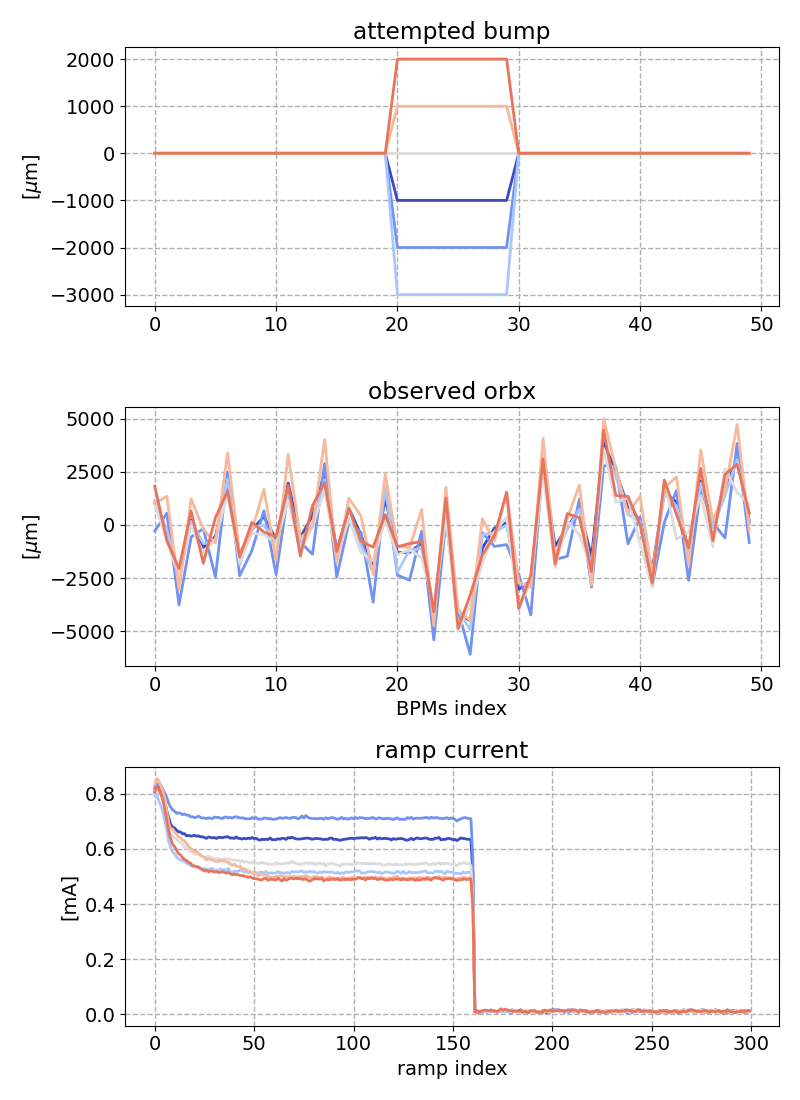
\includegraphics[height=0.9\textheight]{2024-07-12/figures/orbits_and_rampcurr_vs_bumps.png}
\end{minipage} 
\end{frame}


\begin{frame}{Bump de órbita no booster: variações de freq. RF}
\begin{minipage}{0.39\textwidth}
{\footnotesize
\begin{itemize}
    \item estudo do 2024-06-18 \href{https://cnpemcamp.sharepoint.com/:b:/s/FAC/EVB6kJl7jAZHgoUxKpIutQABaUAl3s8RLa3O1rui_7JApg?e=V9X4Yf}{\beamergotobutton{Teams FAC/Machine Studies/Files}}
    \item variações de freq. 
    \item sem efeito na eficiência a não ser p/ variações extremas
    \item investigação de efeitos de carga usando as screens da TB e BO foi abortado por problemas de controle.
\end{itemize}}
% \hsfill
\end{minipage}
\begin{minipage}{0.58\textwidth}
    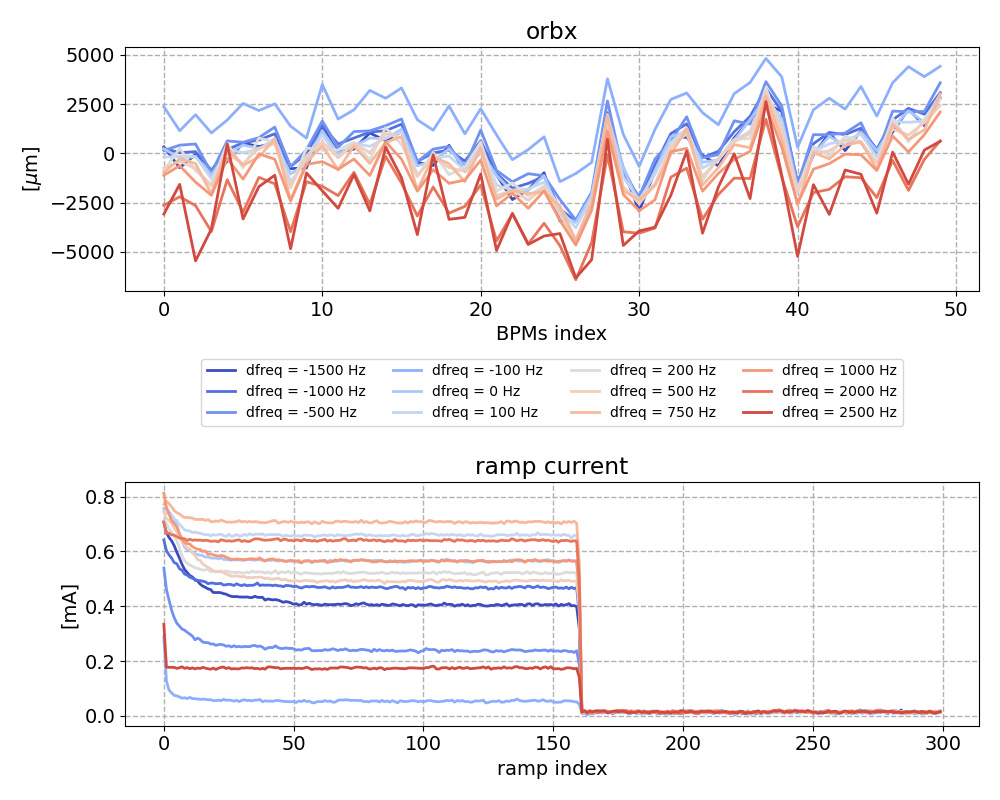
\includegraphics[width=\linewidth]{2024-07-12/figures/orbits_and_rampcurr_vs_dfreq.png}
\end{minipage} 
\end{frame}
% 
\section{Caracterização do linac}

% * 2024-06-24-BO_injector_characterization_and_optimization (li-characterization)


\begin{frame}{Caracterização do linac}

{\footnotesize
\begin{itemize}
    % \setlength\itemsep{1em}
    \item Estudos em 2024-06-24. A ideia era tentar otimizar o Booster mas ... Eficiência de captura muito variável!
    \item Olhando variação do feixe nas screens do Booster migramos para caracterização do Linac
    \item Medimos emitância em alta (3 nC, bias -30.4V) e média carga (1.2 nC, bias -33.4V) do EGun
    \item Otávio irá mudar o foco do trabalho: correção do bump na órbita do BO $\rightarrow$ otimização do LI.
\end{itemize}
}
\begin{figure}[ht]
    \begin{minipage}[b]{0.4\linewidth}
        \centering
        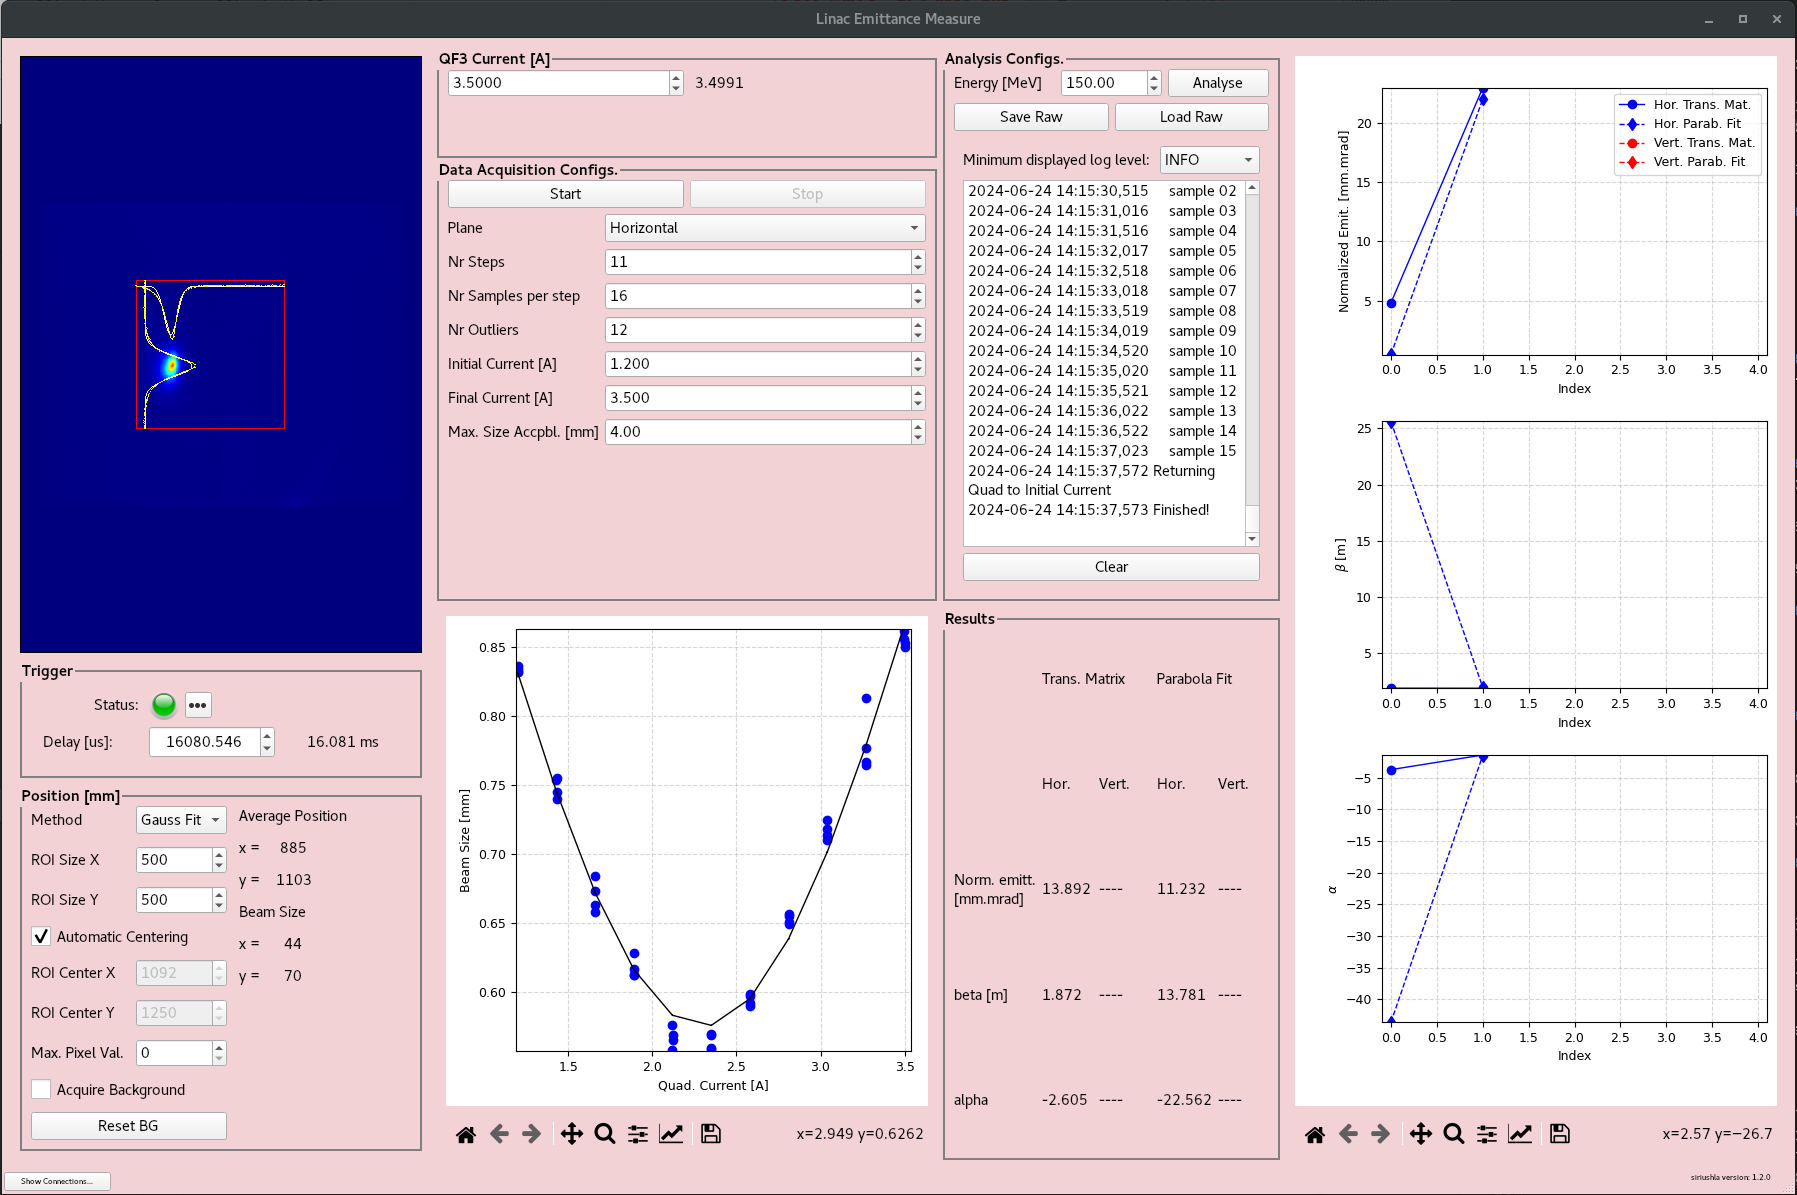
\includegraphics[width=\textwidth]{2024-07-12/figures/emitx_meas_bias_m30p4_charge_3p0nc.png}
        \caption{3 nC Horizontal Emitt.}
        \label{fig:a}
    \end{minipage}
    \hspace{0.3cm}
    \begin{minipage}[b]{0.4\linewidth}
        \centering
        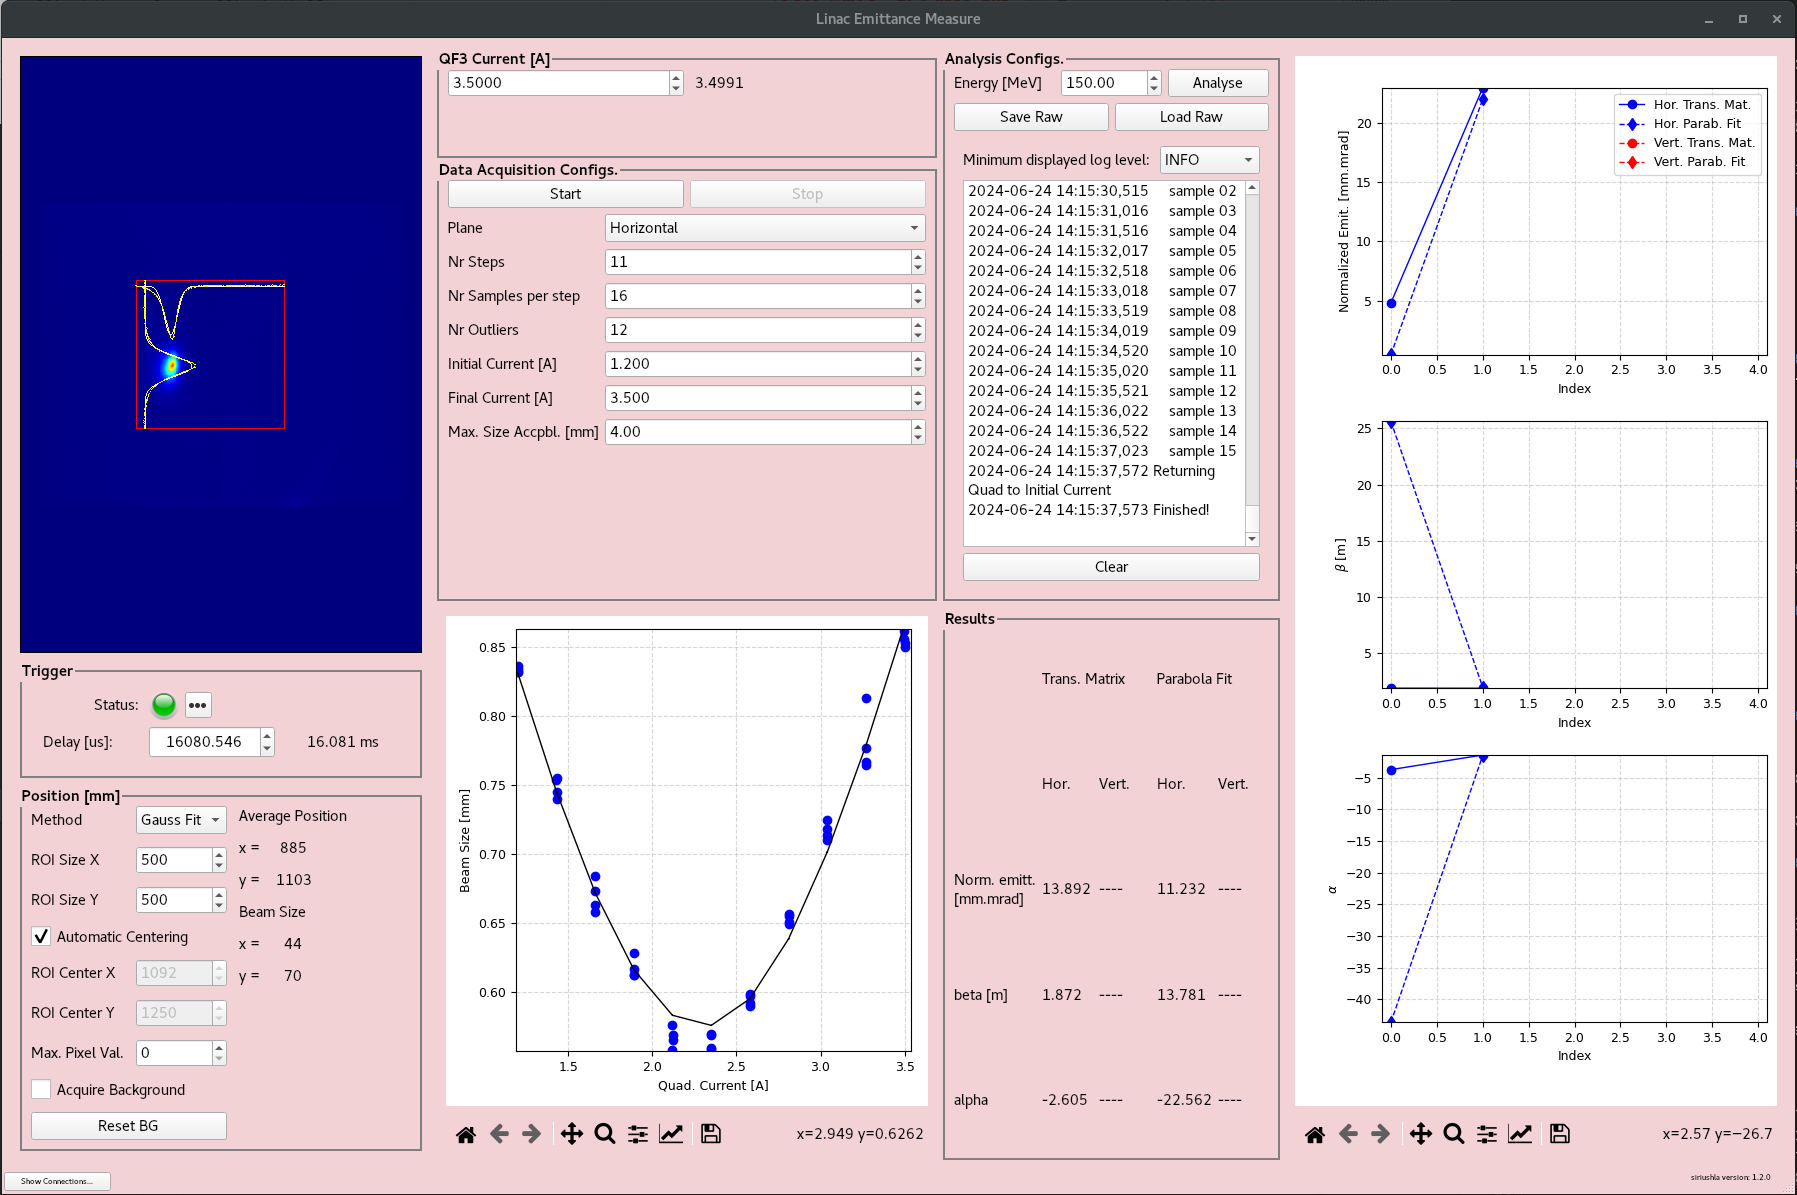
\includegraphics[width=\textwidth]{2024-07-12/figures/emitx_meas_bias_m30p4_charge_3p0nc.png}
        \caption{1.2 nC Horizontal Emitt.}
        \label{fig:b}
    \end{minipage}
\end{figure}
\end{frame}

% % \section{Projeto de Estágio: Correção de Órbita do Booster}

\begin{frame}{Bump de órbita no booster: projeto de estágio}

{\footnotesize
\begin{itemize}
    \item órbita fechada horizontal do booster possui bump ao longo da rampa
    \item correção da órbita ao longo da rampa deslocando QFs (limitado a 1 mm)
    \item ordenamento dos dipolos na instalação descartado como origem principal do bump
    \item relatório parcial apresentado no dia 2024-06-28 \href{https://cnpemcamp.sharepoint.com/:b:/s/FAC/EXHX-vKXStlBipKibZKZwh0BrcXlnEde5HUisWytbQWBog?e=5sYyjp}{\beamergotobutton{Link}}
\end{itemize}
}
% \hsfill
\vspace{0.5cm}
\begin{minipage}{0.49\textwidth}
    \centering
    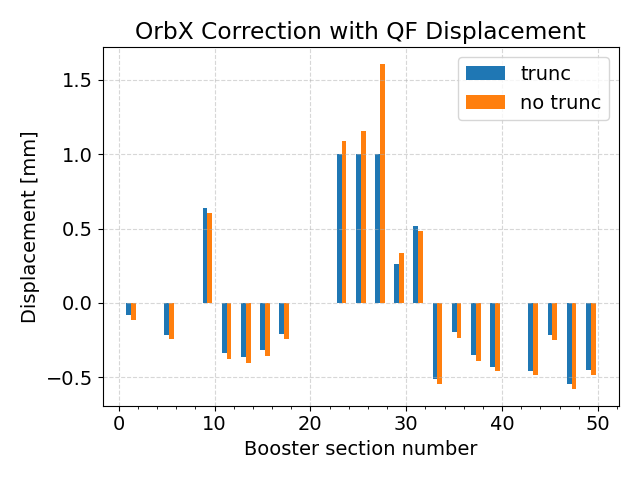
\includegraphics[width=0.8\textwidth]{2024-07-12/figures/qf_displacement_limit.png}
\end{minipage}
\begin{minipage}{0.49\textwidth}
    \centering
    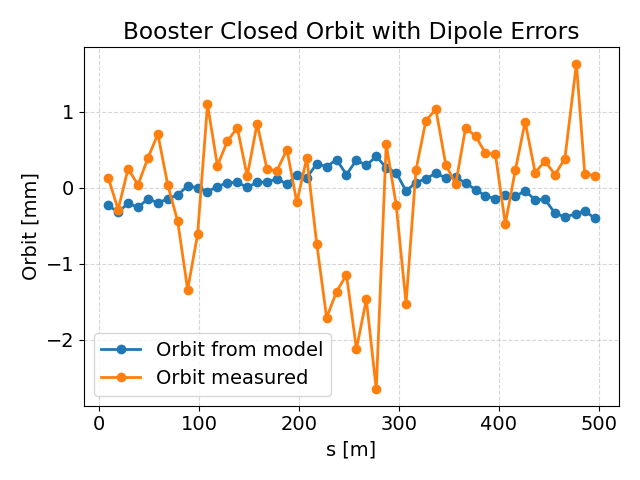
\includegraphics[width=0.8\linewidth]{2024-07-12/figures/orbitx_dipoles_errors.png}
\end{minipage}%
\end{frame}


% \begin{frame}{Projeto de Estágio: Correção de Órbita do Booster}

% {\footnotesize
% \begin{itemize}
%     \item Testar o efeito de correção de órbita utilizando outras órbitas de referência
%     \item Bump não gera nenhum efeito na correção de órbita
%     \item Órbita fica mais deformada
% \end{itemize}
% }
% 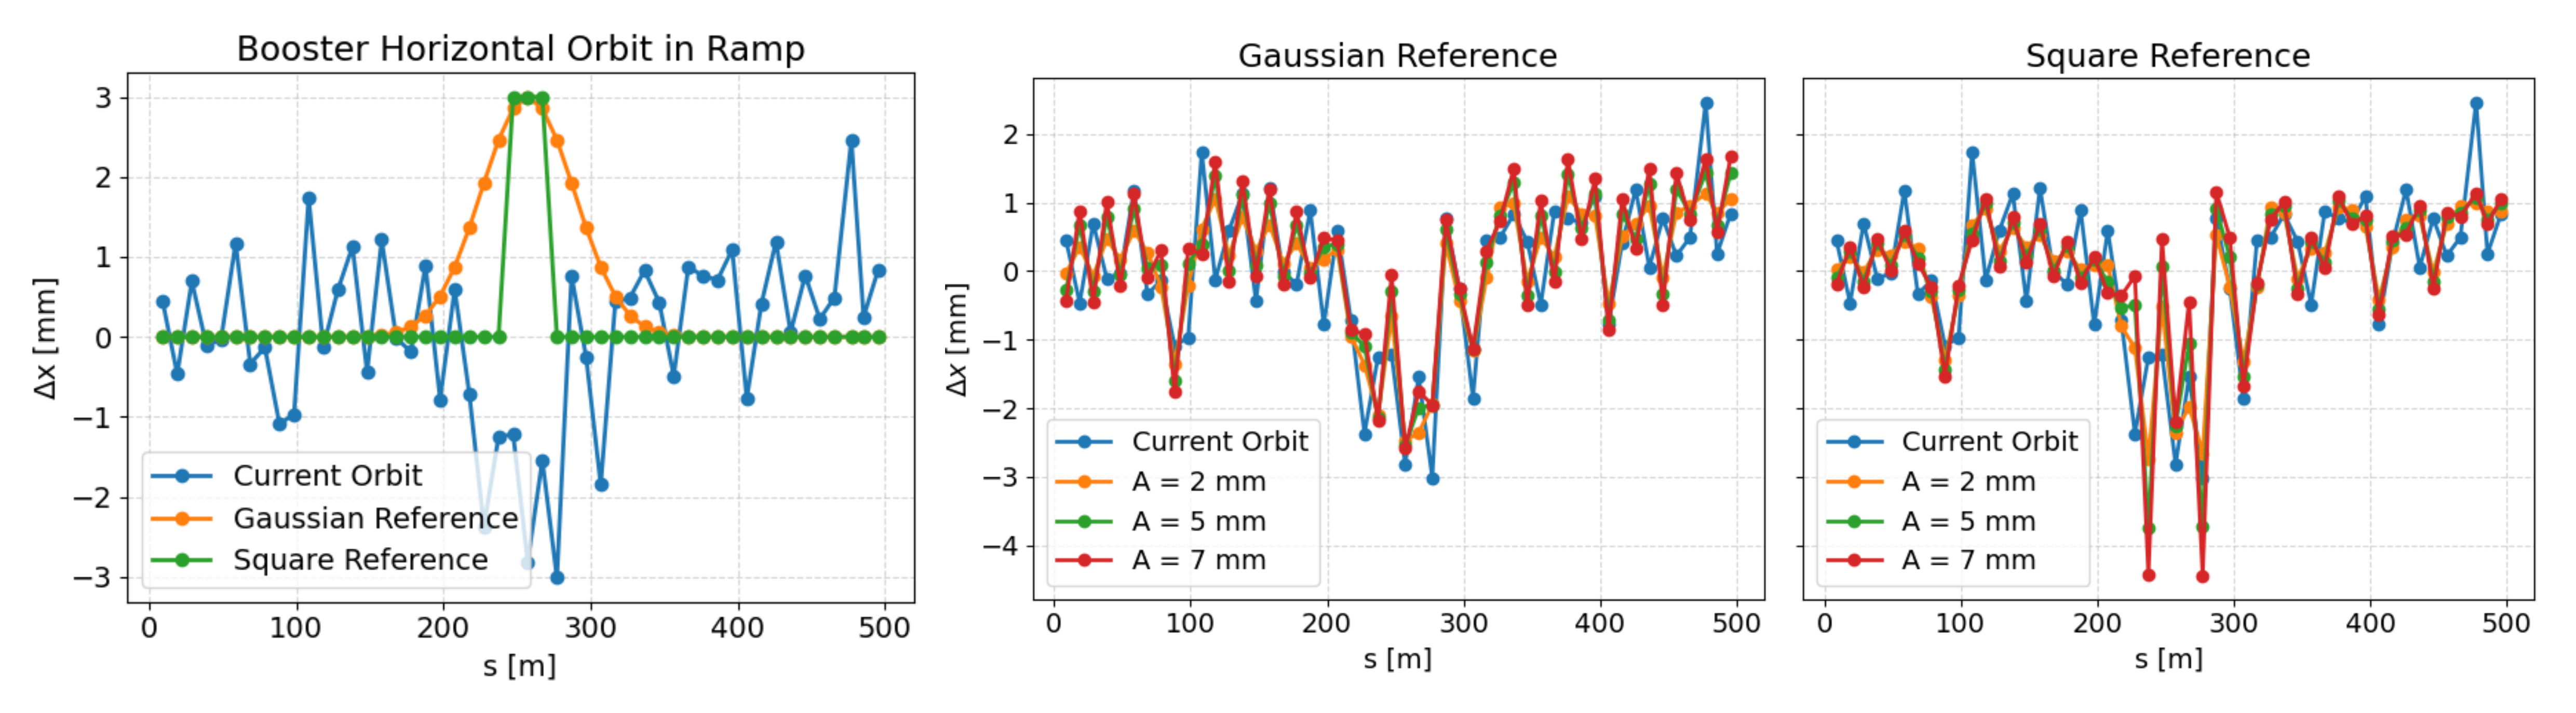
\includegraphics[width=\linewidth]{2024-07-12/figures/bump_types.png}

% \end{frame}


% \begin{frame}{Projeto de Estágio: Correção de Órbita do Booster}

% {\footnotesize
% \begin{itemize}
%     \item Ao serem instalados no Booster, os dipolos foram ordenados propositalmente, de forma que seus erros de campo dipolar estão correlacionados.
%     \item Esses erros foram introduzidos no modelo para ver como afetam o formato da órbita
% \end{itemize}
% }
% \begin{minipage}{0.49\textwidth}
%     \centering
%     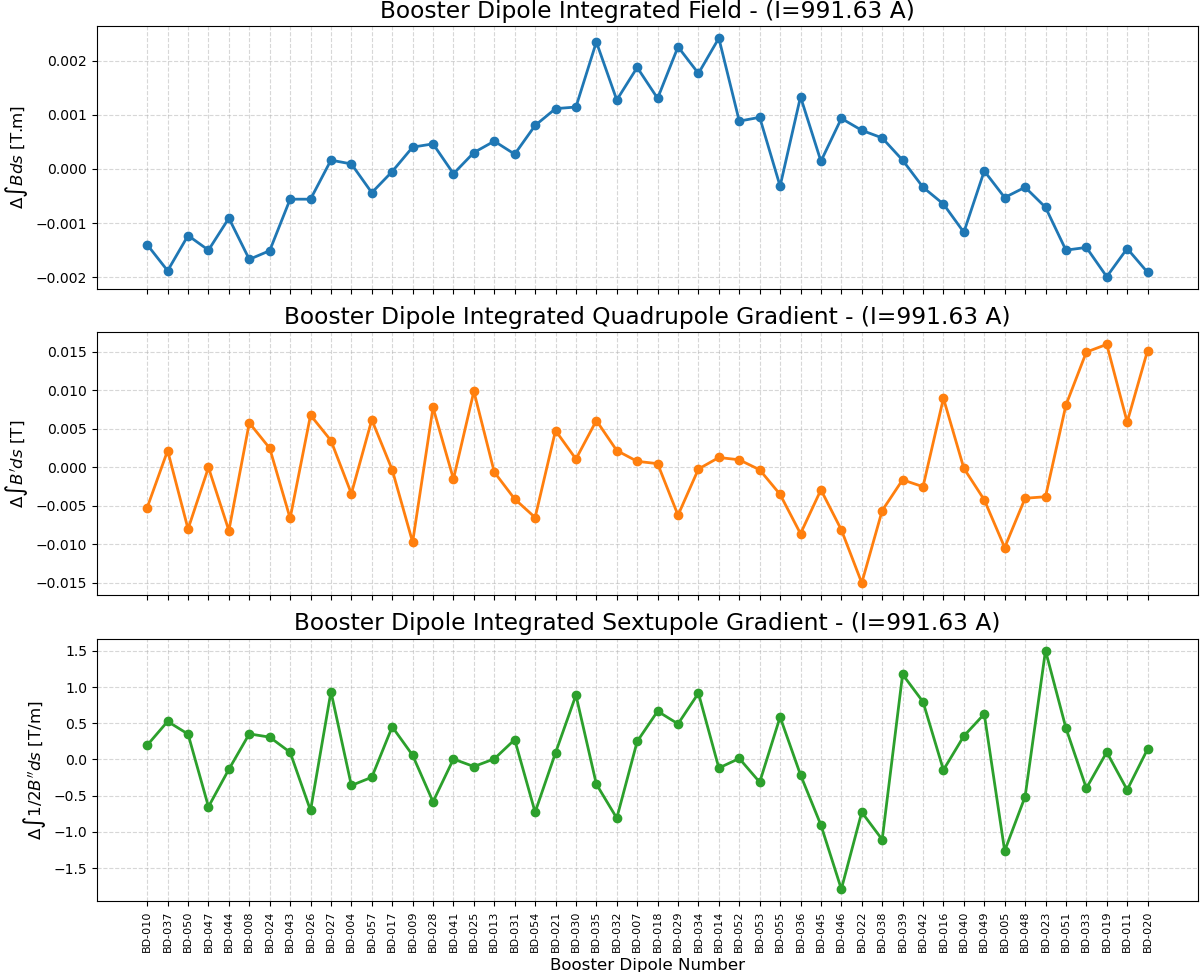
\includegraphics[width=0.9\linewidth]{2024-07-12/figures/dipole_field_sorting.png}
% \end{minipage}%
% \begin{minipage}{0.49\textwidth}
%     \centering
%     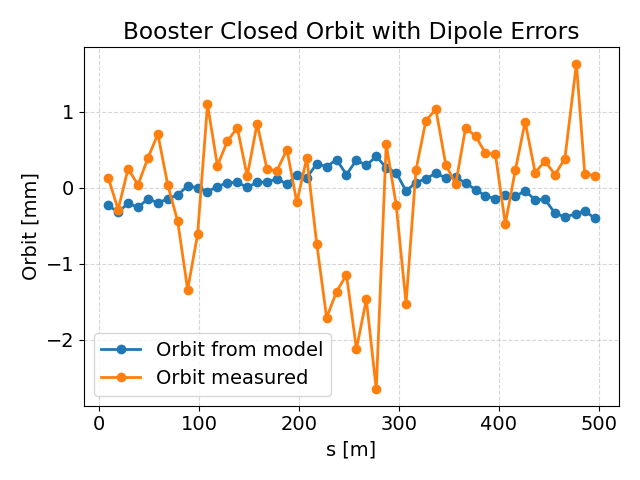
\includegraphics[width=0.8\linewidth]{2024-07-12/figures/orbitx_dipoles_errors.png}
% \end{minipage}
% \end{frame}
% \section{Script de desligamento de máquina}

% * 2024-06-30-AS_machine_shutdown (mac-shutdown)
% * 2024-07-08-AS_machine-startup (mac-shutdown)


\begin{frame}{Script de desligamento de máquina}
\begin{itemize}
    \setlength\itemsep{1em}
    \item Usado em dois domingos, 2024-06-30 e 2024-07-08
    \item O script finalizou desligando todos os subsistemas mas ... alguns problemas nos dois dias
        \begin{itemize}
            \setlength\itemsep{1em}
            \item Timeout (3 min!) no ajuste da tensão de referência da RF do Anel (60 mV)
            \item A PV que registra o tempo que falta para as 6h até o acesso ao túnel está congelada.
            \item Os prints de status durante os comandos de cada subsistema ficam visíveis só ao final do comando, não durante cada etapa.
        \end{itemize}
    \item Reunião marcada entre FAC / SWC / ARO para próxima semana para arredondar as coisas.
\end{itemize}
\end{frame}

% \section{Pyacal}

% * 2024-07-01-SI_pyacal_tests (pyacal-tests)


% \begin{frame}{Pyacal - Testes}
% \begin{itemize}
%     \setlength\itemsep{1em}
%     \item Testes em 2024-07-01
% \end{itemize}
% \end{frame}


% https://indico.desy.de/event/43233/

\begin{frame}{PyACAL}
{\footnotesize
\url{https://github.com/python-accelerator-middle-layer/pyacal-test}
\url{https://github.com/lnls-sirius/pyacal}
}
    \begin{itemize}
        \setlength\itemsep{1em}
        \item Workshop no DESY sobre Accelerator Middle Layer (2024-06-2024) \href{https://indico.desy.de/event/43233/}{\beamergotobutton{Link}}
        \item Apresentação do Fernando sobre nossa experiência com Python 
        % \href{https://cnpemcamp.sharepoint.com/:p:/s/FAC/EQwEQKO9bsFJlqgcFRk-43ABjphWKXvMnEUq9Mn3pOGc-w?e=sFLhcV&clickparams=eyJBcHBOYW1lIjoiVGVhbXMtRGVza3RvcCIsIkFwcFZlcnNpb24iOiIxNDE1LzI0MDYyODA2NDAwIiwiSGFzRmVkZXJhdGVkVXNlciI6ZmFsc2V9}{\beamergotobutton{Link}}
        \href{https://indico.desy.de/event/43233/contributions/169377/attachments/90992/122797/SIRIUS_python_code.pdf}{\beamergotobutton{Link}}
        
        \item Accelerator Control Abstraction Layer (PyACAL)
            \begin{itemize}
                \item Accelerator Digital Twin (Online \& Simul)
                \item Devices $\rightarrow$ experiments
            \end{itemize}
        \item Zoom meeting em 2024-06-28 (Sirius/Soleil/Desy/ESRF/Diamond...)
        \item Testes no dia 2024-07-01
            \begin{itemize}
                \item Orbit Response Matrix Measurement (ok!)
                \item BBA (parcial...)
                \item Chromaticity \& Dispersion measurement (não testado)
            \end{itemize}
    \end{itemize}
\end{frame}

\end{document}
